\documentclass{article}
\usepackage{graphicx}
\usepackage[margin=1.5cm]{geometry}
\usepackage{amsmath}

\begin{document}

\title{Monday Reading Assessment: Unit 5, Field Induction and Inductance}
\author{Prof. Jordan C. Hanson}

\maketitle

\section{Memory Bank}

\begin{itemize}
\item $M = \frac{N\phi}{I}$ ... Definition of mutual inductance.
\item $\epsilon = -M dI/dt$ ... Relationship between induced voltage and inductance, and changing in current.
\item $M_{21} = (N_2 \phi_{21})/I_1$ ... Mutual inductance in solenoid 2 due to solenoid 1 with current 1.
\item $P = i\epsilon$ ... Power is current times voltage.
\end{itemize}

\section{Mutual Inductance}

\begin{figure}
\centering
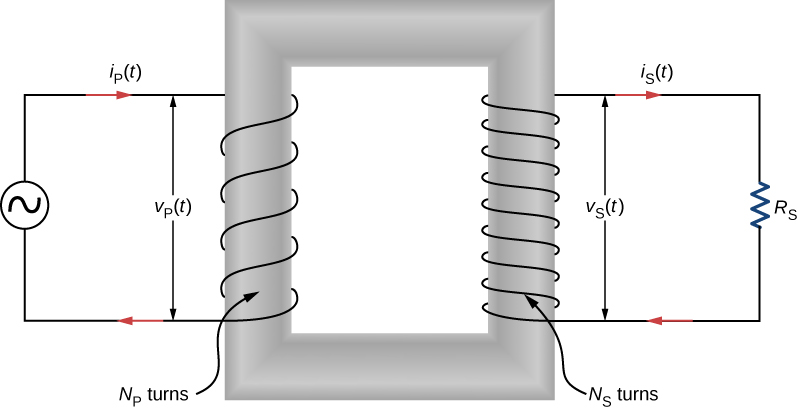
\includegraphics[width=0.5\textwidth]{transform.jpeg}
\caption{\label{fig:trans} A cross-sectional view of a solenoid.}
\end{figure}

\begin{enumerate}
\item Consider Fig. \ref{fig:trans}, in which two solenoids are \textit{ideally} coupled with an iron core.  \textit{Ideally} means that $\phi_{12} = \phi_{21}$, and this occurs because of the properties of iron atoms.  Let solenoid P have $N_1$ turns, and AC voltage $\epsilon_1$, while solenoid 2 has $N_2$ turns, and AC voltage $\epsilon_2$.  Show that 
\begin{equation}
\frac{\epsilon_2}{\epsilon_1} = \frac{N_2}{N_1}
\end{equation} \\ \vspace{1cm}
\item If the maximum voltage of $\epsilon_1(t)$ is 2 kV, with $N_1 = 1000$ turns, and we want the maximum of $\epsilon_2(t)$ to be 120 V, how many turns should we put in solenoid S? \\ \vspace{1.5cm}
\item Since energy has to be conserved, the power flowing into the transformer has to equal the power flowing out.  Convince yourself that
\begin{equation}
i_P \epsilon_P = i_S \epsilon_S
\end{equation}
If the current flowing into the transformer is 2.0 A, what current flows out?
\end{enumerate}
\end{document}
